\section{Kanalzuteilung, Fehlerkorrektur}

\subsection{Zugriffsverfahren}

\begin{defi}{Zugriffsverfahren}
    Über das \emph{Zugriffsverfahren} wird der Medienzugriff in Netzwerken festgelegt.

    Im OSI-Modell wird darunter die Kommunikation zwischen dem Physical Layer (Schicht 1, Bitübertragungsschicht) und dem MAC-Layer (Schicht 2a, Teil der Sicherungsschicht) verstanden.

    Über das Zugriffsverfahren wird geregelt, welche Station zu welchem Zeitpunkt welche Datenmenge an wen übertragen darf.

    Im LAN ist wichtig festzulegen, wie die beteiligten Stationen und Netzkomponenten auf das Netzwerkkabel zugreifen.
    Die Regelung des Zugriffs und die damit verknüpfte Übertragung von geeigneten Daten in einem festgelegten Rahmen, gehören zu den Hauptaufgaben des MAC-Layers.
\end{defi}

\begin{defi}{TDMA}
    Beim \emph{Zeitmultiplexverfahren} bzw. \emph{Time Division Multiple Access (TDMA)} werden in bestimmten Zeitabschnitten  die Daten (Signale) verschiedener Sender auf einem Kanal übertragen.
\end{defi}

\begin{defi}{FDMA}
    Das \emph{Frequenzmultiplexverfahren} bzw. \emph{Frequency Division Multiple Access (FDMA)}  ist ein nachrichtentechnisches Multiplexverfahren, mit dem gleichzeitig mehrere Signale auf mehrere Träger verteilt übertragen werden können.

    Die Träger sind mehreren unterschiedlichen Frequenzen zugeordnet.
\end{defi}

\begin{defi}{CDMA}
    Das \emph{Codemultiplexverfahren} bzw. \emph{Code Division Multiple Access (CDMA)} ist ein Multiplexverfahren, das die gleichzeitige Übertragung verschiedener Nutzdatenströme auf einem gemeinsamen Frequenzbereich ermöglicht. Der gemeinsam genutzte Frequenzbereich weist dabei als wesentliche Eigenschaft eine größere Bandbreite auf, als der Nutzdatenstrom belegt.

    Zur Unterscheidung werden die Datenströme mit speziellen \enquote{Spreizcodes} codiert, wobei diese Codefolgen zusätzlich bestimmte Eigenschaften wie Orthogonalität aufweisen und in bestimmten Anwendungen auf Pseudozufall basieren, wodurch auf Empfängerseite durch Korrelation mit der Spreizcodefolge die ursprünglichen Nutzdatenströme voneinander getrennt gewonnen werden können.

    Gegenüber den klassischen Multiplexverfahren wie dem Frequenzmultiplex und dem Zeitmultiplex erfolgt bei dem Codemultiplex eine Überlagerung der einzelnen Datenströme sowohl im Frequenzbereich als auch im Zeitbereich.
\end{defi}

\begin{defi}{CSMA}
    \emph{Carrier Sense Multiple Access (CSMA)} bezeichnet ein dezentrales, asynchrones Verfahren zum Erlangen des Zugriffsrechts nach dem Konkurrenzverfahren auf Busleitungen.

    Trägerprüfung bzw. Carrier Sense bedeutet, dass alle Teilnehmer den Status der Busleitung beobachten und ihre Nachrichten nur senden, wenn gerade kein anderer Teilnehmer sendet, der Kanal also frei ist.

    Ist das Medium für eine bestimmte Zeitspanne\footnote{9,6 $\mu$s bei 10-Mbps-Ethernet, 960 ns bei 100-Mbps-Fast-Ethernet und 96 ns bei 1000 Mbps} nicht belegt, wird es als frei betrachtet.

    Kollisionen können eintreten, wenn zwei oder mehr Teilnehmer gleichzeitig mit dem Senden beginnen.
\end{defi}

\begin{defi}{CSMA/CD}
    \emph{Carrier Sense Multiple Access/Collision Detection (CSMA/CD)} ist eine Erweiterung von CSMA.
    Verwendung findet CSMA/CD z.B. bei Ethernet.\footnote{ Bei Wireless LANs wird ein deutlich anderer Mechanismus namens Carrier Sense Multiple Access/Collision Avoidance (CSMA/CA) benutzt.}

    Wenn ein Gerät Daten senden möchte, hält es sich an folgenden Ablauf:
    \begin{enumerate}
        \item \emph{Horchen}: Zuerst muss das Medium überwacht werden, ob es belegt ist.
              \begin{itemize}
                  \item Frei: Wenn das Medium eine bestimmte Zeit lang frei ist, weiter mit Schritt 2.
                  \item Belegt: Weiter mit Schritt 1.
              \end{itemize}
        \item \emph{Senden}: Informationsübertragung, zugleich wird das Medium fortwährend weiter abgehört.
              \begin{itemize}
                  \item Erfolg (keine Kollision bis Übertragungsende): Übertragung ist erfolgreich abgeschlossen und es wird eine Erfolgsmeldung an höhere Netzwerkschichten gemeldet; weiter mit Schritt 5.
                  \item Kollision: Wird eine Kollision entdeckt, beende die Datenübertragung und sende ein kurzes, definiertes Störsignal (\emph{jam}) auf die Leitung, um sicherzustellen, dass alle anderen Transceiver die Kollision ebenfalls erkennen, dann weiter mit Schritt 3.
              \end{itemize}
        \item \emph{Leitung ist belegt}: Überprüfung der Anzahl der Übertragungsversuche:
              \begin{itemize}
                  \item Maximum nicht erreicht: Eine zufällige Zeit (\emph{Backoff}) abwarten, dann wieder bei Schritt 1 beginnen.
                  \item Maximum erreicht: Weiter mit Schritt 4.
              \end{itemize}
        \item \emph{Fehler}: Maximale Anzahl von Übertragungsversuchen wurde überschritten. Ein Fehler wird an die höheren Netzwerkschichten gemeldet, weiter mit Schritt 5.
        \item \emph{Ende}: Übertragungsmodus verlassen
    \end{enumerate}
\end{defi}

\begin{diag}{CSMA/CD}
    \centering
    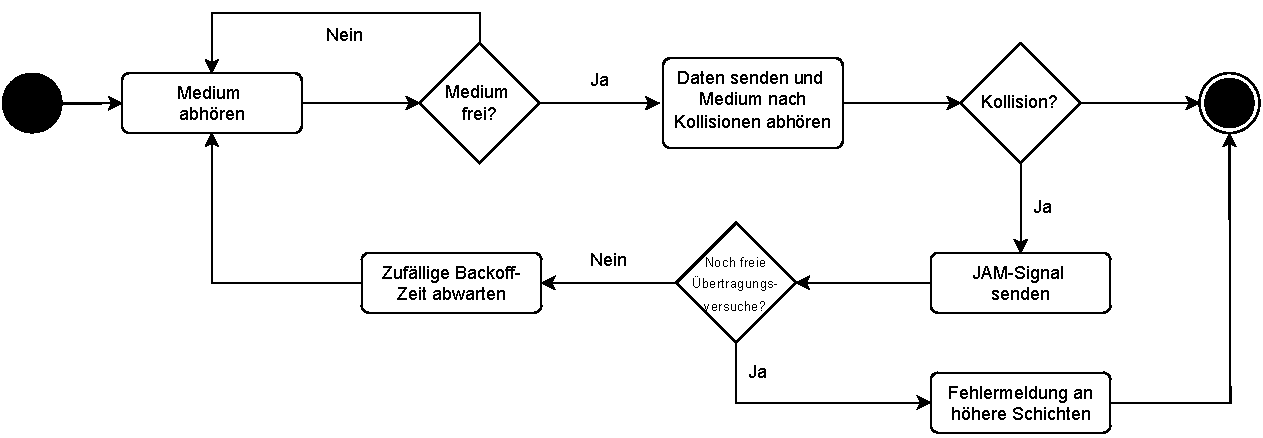
\includegraphics[width=\textwidth]{includes/figures/defi_csmacd.pdf}
\end{diag}

\subsection{Ethernet}

\begin{defi}{Ethernet}
    \emph{Ethernet} ist eine Technik, die Software (Protokolle usw.) und Hardware (Kabel, Verteiler, Netzwerkkarten usw.) für kabelgebundene Datennetze spezifiziert, welche ursprünglich für lokale Datennetze (LANs) gedacht war.

    Sie ermöglicht den Datenaustausch in Form von Datenframes zwischen den in einem lokalen Netz (LAN) angeschlossenen Geräten.

    Im OSI-Modell ist mit Ethernet sowohl die physische Schicht (OSI Layer 1) als auch die Data-Link-Schicht (OSI Layer 2) festgelegt.

    Ethernet verwendet CSMA/CD.
    Bei Kollisionen wird Binary Exponential Backoff verwendet.
\end{defi}

\begin{defi}{Binary Exponential Backoff}
    Der \emph{Binary Exponential Backoff} ist ein Stauauflösungsmechanismus im Ethernet.

    Wird von Stationen im Ethernet eine Kollision erkannt, beenden diese Stationen ihre Sendung und versuchen sofort oder nach einer Slot-Time von 51.2 $\mu$s\footnote{entspricht 512 Bit, gilt nur für 10/100 MBit/s Ethernet, 4,096 $\mu$s und 4096 Bit bei 1 GBit/s} erneut ihre Sendung über das Ethernet zu übertragen.
    Dabei kann es erneut zu einer Kollision kommen, wenn beide Stationen zufällig die gleiche Wahl treffen.

    Beim nächsten Versuch wird nun jede der beiden Stationen wieder per Zufallsentscheidung einen neuen Starttermin auswählen, diesmal aber aus vier Möglichkeiten: 0, 1, 2 oder 3 Slot-Times, also $2^2$.

    Bei einer erneuten Kollision sind es dann $2^3 = 8$ Möglichkeiten, dann 16, 32, 64, 128, 256, 512 und schließlich 1024 ($2^{10}$), was auch die Maximalgrenze der Möglichkeiten darstellt.

    Nach insgesamt 16 erfolglosen Übertragungsversuchen mit Kollision wird mit einer Fehlermeldung des Ethernet-Controllers abgebrochen.
\end{defi}

\begin{defi}{Ethernet-Frame}
    \centering
    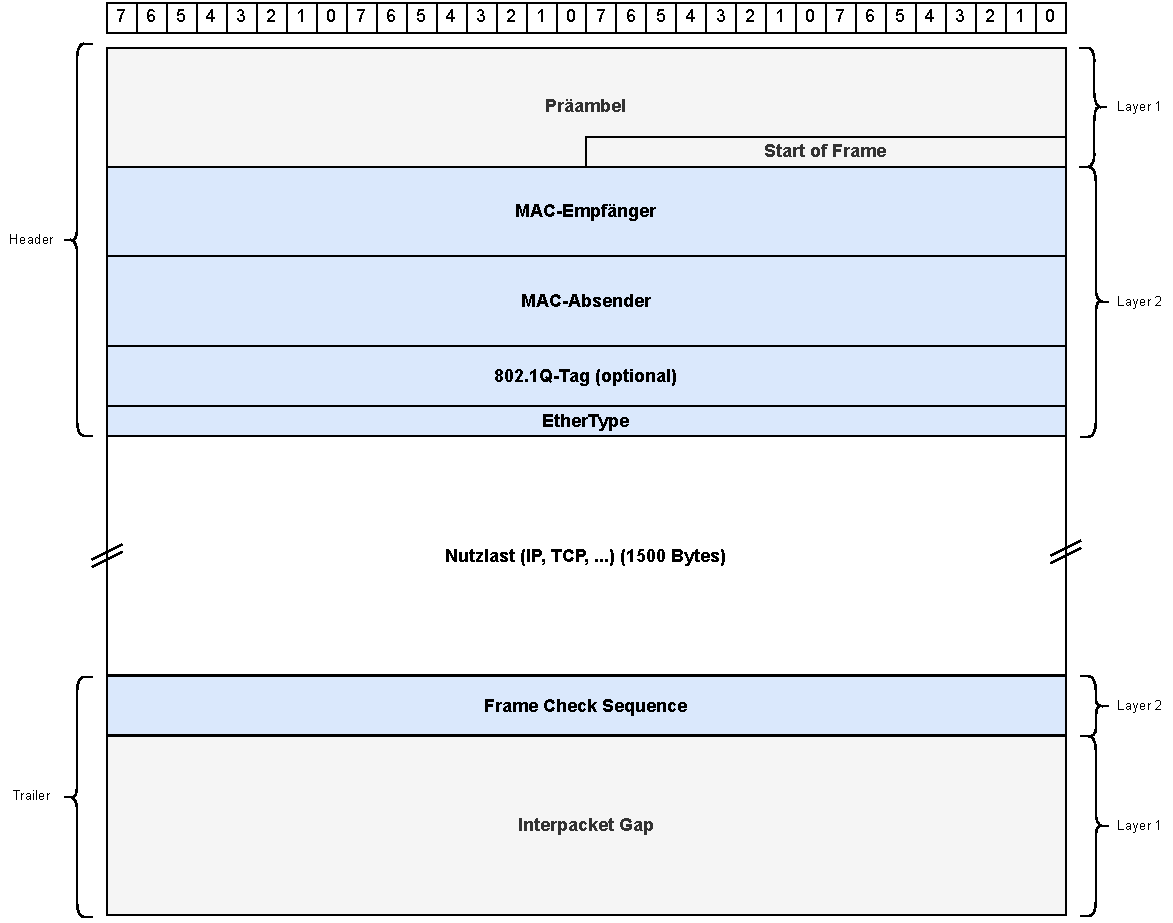
\includegraphics[width=.9\textwidth]{includes/figures/defi_ethernet_frame.pdf}
\end{defi}

\begin{bonus}{Token-Ring}
    \emph{Token-Ring} ist eine Vernetzungstechnik für Computernetzwerke.

    Die Token-Ring-Technik wurde praktisch vollständig von den verschiedenen Ethernet-Varianten verdrängt.

    Ein Token kreist bei Token-Ring-Netzen über den Ring: Das Token wird stets von einem Knoten an den nächsten weitergereicht.\footnote{Selbst im Leerlauf geben die Stationen das Paket fortwährend weiter.}

    Möchte nun ein Computer Daten versenden, wartet er, bis das Token ihn erreicht hat, dann hängt er seine Nutzdaten daran an.
    Zugleich ergänzt er das Token um Steuersignale und setzt außerdem das Token-Bit von 0 (für \enquote{freies Token}) auf 1, aus dem Frei-Token wird also ein Datenrahmen.

    Jeder Rechner prüft, ob das Paket an ihn adressiert ist, und setzt es anderenfalls zurück auf den Ring.
    Erhält der vorgesehene Empfänger den an ihn adressierten Datenrahmen, kopiert er die Nutzdaten und quittiert den Datenempfang.

    Der Sender erhält die Quittung und sendet das Token mit den nächsten Nutzdaten oder setzt ein Frei-Token auf den Ring.
\end{bonus}

\subsection{Fehlererkennung}

\begin{defi}{Hamming-Abstand}
    Der \emph{Hamming-Abstand} bzw. \emph{Hamming-Distanz} sind Maße für die Unterschiedlichkeit von Zeichenketten.

    Der Hamming-Abstand zweier Blöcke mit fester Länge (sogenannter Codewörter) ist dabei die Anzahl der unterschiedlichen Stellen.

    Es wird zur Fehlererkennung und zur Fehlerkorrektur benutzt, indem Dateneinheiten, die über eine Übertragungsstrecke empfangen werden, mit gültigen Zeichen verglichen werden.

    Eine etwaige Korrektur der Zeichen erfolgt nach dem Wahrscheinlichkeitsprinzip.
    Ob eine Fehlererkennung oder -korrektur stattfinden kann, hängt von der Hamming-Distanz ab.
\end{defi}

\begin{defi}{Wiederholung Hamming-Codierung}
    Bei der \emph{Hamming-Codierung} werden Paritätsinformationen zu Daten hinzugefügt, um so mögliche Übertragungsfehler zu erkennen.

    Hamming-Codewörter haben die Länge $N = 2^k-1$, wobei $k$ Paritätsbits enthalten sind.
    Die Bits werden der Einfachheit halber bei Eins beginnend durchnummeriert.

    Die Paritätsbits stehen an den Stellen, deren Index eine 2er-Potenz ist.\footnote{Sehr empfehlenswert: \href{https://youtu.be/X8jsijhllIA}{3Blue1Brown: How to send a self-correcting message (Hamming codes)}}

    Sind $p_1, p_2, \ldots, p_k$ Paritätsbits, $d_1, d_2, \ldots, d_{N-k}$ Bits des Datenwortes und $c_1, c_2, \ldots, c_N$ die Bits des zu bildenden Codewortes, hat ein Codewort des so konstruierten Hamming-Codes die folgende Form:

    \begin{tabular}{| c | c | c || c | c | c | c || c | c | c | c | c | c | c | c || c | c | c |}
        \hline
        $c_1$ & $c_2$ & $c_3$ & $c_4$ & $c_5$ & $c_6$ & $c_7$ & $c_8$ & $c_9$ & $c_{10}$ & $c_{11}$ & $c_{12}$ & $c_{13}$ & $c_{14}$ & $c_{15}$ & $c_{16}$ & $c_{17}$ & \ldots \\
        \hline
        \hline
        $p_0$ & $p_1$ & $d_1$ & $p_2$ & $d_2$ & $d_3$ & $d_4$ & $p_3$ & $d_5$ & $d_6$    & $d_7$    & $d_8$    & $d_9$    & $d_{10}$ & $d_{11}$ & $p_4$    & $d_{12}$ & \ldots \\
        \hline
    \end{tabular}\\

    Dabei wird jedem Paritätsbit eine spezielle Bitmaske zugewiesen:

    \begin{tabular}{| c || c | c | c || c | c | c | c || c | c | c | c | c | c | c | c || c |}
        \hline
        Bitmaske & $c_1$ & $c_2$ & $c_3$ & $c_4$ & $c_5$ & $c_6$ & $c_7$ & $c_8$ & $c_9$ & $c_{10}$ & $c_{11}$ & $c_{12}$ & $c_{13}$ & $c_{14}$ & $c_{15}$ & \ldots \\
        \hline
        \hline
        $p_0$    & $p_0$ & $p_1$ & 1     & $p_2$ & 1     & 0     & 1     & $p_3$ & 1     & 0        & 1        & 0        & 1        & 0        & 1        & \ldots \\
        $p_1$    & $p_0$ & $p_1$ & 1     & $p_2$ & 0     & 1     & 1     & $p_3$ & 0     & 1        & 1        & 0        & 0        & 1        & 1        & \ldots \\
        $p_2$    & $p_0$ & $p_1$ & 0     & $p_2$ & 1     & 1     & 1     & $p_3$ & 0     & 0        & 0        & 1        & 1        & 1        & 1        & \ldots \\
        $p_3$    & $p_0$ & $p_1$ & 0     & $p_2$ & 0     & 0     & 0     & $p_3$ & 1     & 1        & 1        & 1        & 1        & 1        & 1        & \ldots \\
        \hline
    \end{tabular}\\

    Damit gilt:
    $$
        \begin{aligned}
            c_1 = p_0 & = c_3 \oplus c_5 \oplus c_7 \oplus c_9 \oplus c_{11} \oplus c_{13} \oplus c_{15} \oplus \ldots    \\
                      & \iff \text{jedes ungerade Datenbit}                                                               \\
            c_2 = p_1 & = c_3 \oplus c_6 \oplus c_7 \oplus c_{10} \oplus c_{11} \oplus c_{14} \oplus c_{15} \oplus \ldots \\
                      & \iff \text{ein Datenbit rechts von $p_1$, zwei überspringen, zwei einberechnen, $\ldots$}         \\
            c_4 = p_2 & = c_5 \oplus c_6 \oplus c_7 \oplus c_{12} \oplus c_{13} \oplus c_{14} \oplus c_{15} \oplus \ldots \\
                      & \iff \text{drei Datenbit rechts von $p_2$, vier überspringen, vier einberechnen, $\ldots$}
        \end{aligned}
    $$
\end{defi}

\begin{algo}{Wiederholung Fehlererkennung beim Hamming-Code}
    Situation: Empfangen eines Hamming-codierten Datensatzes

    \begin{enumerate}
        \item Erneutes Berechnen der \emph{Paritätsbits}
        \item Erkennen, welche neu berechneten Paritätsbits $p'_i$ \emph{verschieden} sind zu den empfangenen Paritätsbits $p_i$
        \item Bitfehler ist in dem Datenbit passiert, in dem gilt:
              \subitem $p_i = p'_i \implies$ Bitmaske für $p_i$ ist $0$
              \subitem $p_i \neq p'_i \implies$ Bitmaske für $p_i$ ist $1$
    \end{enumerate}

    Es wird angenommen, dass nur ein Bitfehler in den Datenbits passiert ist.

    Anmerkung: Ist lediglich ein Paritätsbit verschieden, dann ist ein Übertragungsfehler in dem betreffenden Paritätsbit selbst aufgetreten, da alle Datenbits zur Berechnung von mindestens zwei Paritätsbits verwendet werden.
\end{algo}

\begin{defi}{CRC}
    Die \emph{zyklische Redundanzprüfung} (\emph{Cyclic Redundancy Check (CRC)})  ist ein Verfahren zur Bestimmung eines Prüfwerts für Daten, um Fehler bei der Übertragung oder Speicherung erkennen zu können. Im Idealfall kann das Verfahren sogar die empfangenen Daten selbständig korrigieren, um eine erneute Übertragung zu vermeiden.

    Die Bitfolge der Coderepräsentation der Daten wird durch ein vorher festzulegendes Generatorpolynom (das CRC-Polynom) Modulo 2 geteilt, wobei ein Rest bleibt (CRC-Wert).

    Um zu verifizieren, dass die Daten keinen Fehler beinhalten, wird der empfangene Datenblock mit angehängtem CRC-Wert als Binärfolge interpretiert, erneut durch das CRC-Polynom Modulo geteilt und der Rest ermittelt.

    Wenn kein Rest bleibt, ist entweder kein Fehler aufgetreten oder es ist ein (unwahrscheinlicher) Fehler aufgetreten, der in Polynomdarstellung das CRC-Polynom als Faktor hat.
\end{defi}

\begin{example}{CRC (Senden)}
    \setcounter{MaxMatrixCols}{20}
    Gegeben seien:
    \begin{itemize}
        \item Generator- bzw. CRC-Polynom \texttt{110101} ($x^5 + x^4 + x^2 + x^0$).
        \item Rahmen: \texttt{11011}
        \item Rahmen mit Anhang:\footnote{Der zu übertragenden Bitfolge werden $n$ Nullen angehängt, wobei $n$ dem Grad des Polynoms entspricht.} \texttt{1101100000}
    \end{itemize}

    Nun wird der Rahmen mit Anhang von links her durch das Generatorpolynom dividiert:\footnote{Dabei wird ausschließlich \texttt{XOR} verwendet!}

    \[
        \begin{matrix}
                   & 1 & 1 & 0 & 1      & 1 & 0 & 0 & 0 & 0 & 0 &        \\
            \oplus & 1 & 1 & 0 & 1      & 0 & 1 &   &   &   &   &        \\\cline{1-7}
                   &   &   &   &        & 1 & 1 & 0 & 0 & 0 & 0 &        \\
                   &   &   &   & \oplus & 1 & 1 & 0 & 1 & 0 & 1 &        \\\cline{5-11}
                   &   &   &   &        & 0 & 0 & 0 & 1 & 0 & 1 & (Rest)
        \end{matrix}
    \]

    An den Rahmen ohne Anhang wird nun der Rest angehängt.
    Dieser muss ebenfalls aus $n$ Bits bestehen.
    Damit hängen wir nun \texttt{00101} an den Rahmen an.

    Übertragener Rahmen: \texttt{1101100101}

    Diese Nachricht kann jetzt beispielsweise über ein Netzwerk übertragen werden. Wenn die Nachricht beim Empfänger eintrifft, kann dieser überprüfen, ob sie korrekt angekommen ist.
\end{example}

\begin{example}{CRC (Empfangen)}
    \setcounter{MaxMatrixCols}{20}
    Gegeben seien:
    \begin{itemize}
        \item Generator- bzw. CRC-Polynom \texttt{110101} ($x^5 + x^4 + x^2 + x^0$).
        \item Übertragene Nachricht: \texttt{1001100101}
    \end{itemize}

    Wir wollen die Nachricht auf Korrektheit prüfen.
    Es gilt:
    \[
        \begin{matrix}
                   & 1      & 0      & 0      & 1      & 1 & 0 & 0 & 1 & 0 & 1 &        \\
            \oplus & 1      & 1      & 0      & 1      & 0 & 1 &   &   &   &   &        \\\cline{1-7}
                   &        & 1      & 0      & 0      & 1 & 1 & 0 &   &   &   &        \\
                   & \oplus & 1      & 1      & 0      & 1 & 0 & 1 &   &   &   &        \\\cline{2-8}
                   &        &        & 1      & 0      & 0 & 1 & 1 & 1 &   &   &        \\
                   &        & \oplus & 1      & 1      & 0 & 1 & 0 & 1 &   &   &        \\\cline{3-9}
                   &        &        &        & 1      & 0 & 0 & 1 & 0 & 0 &   &        \\
                   &        &        & \oplus & 1      & 1 & 0 & 1 & 0 & 1 &   &        \\\cline{4-10}
                   &        &        &        &        & 1 & 0 & 0 & 0 & 1 & 1 &        \\
                   &        &        &        & \oplus & 1 & 1 & 0 & 1 & 0 & 1 &        \\\cline{5-11}
                   &        &        &        &        &   & 1 & 0 & 1 & 1 & 0 & (Rest) \\
        \end{matrix}
    \]

    Der Rest der Division (\texttt{10110}) ist ungleich null. Also ist ein Fehler aufgetreten.
\end{example}